\subsection{Reminders}

\begin{frame}[fragile]{SAS Viya and the AI and Analytics Life Cycle}

\begin{figure}[H]
    \centering
    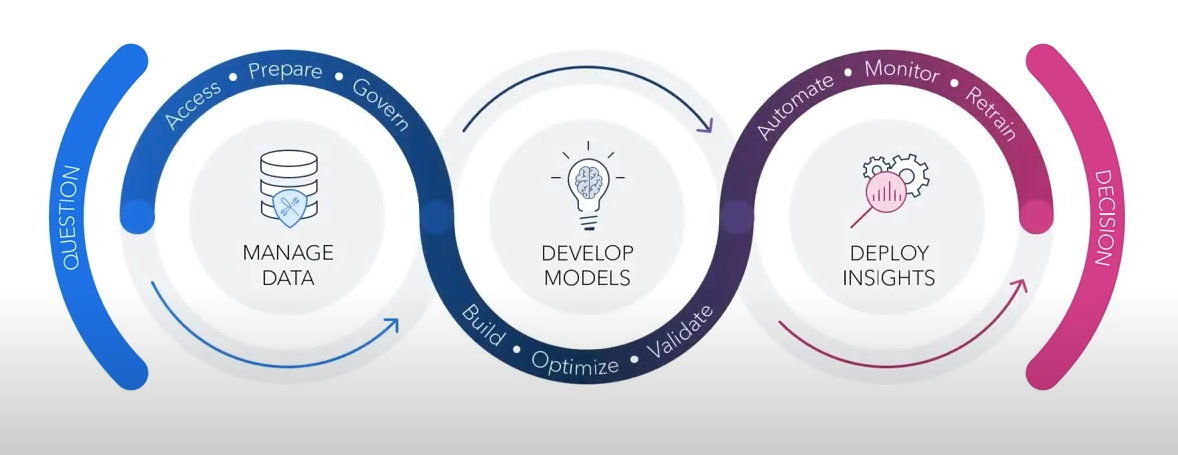
\includegraphics[width=1\linewidth]{Images/life_cycle.png}
\end{figure}


\end{frame}


\begin{frame}[fragile]{The Curse of Dimensionality}
\textbf{Definition:} 
\begin{itemize}
    \item The curse of dimensionality refers to the explosive increase in volume
    (or data sparsity) that occurs when adding extra dimensions to a mathematical space.
\end{itemize}

\vfill

\textbf{Why It Matters:}
\begin{itemize}
    \item \textbf{Data Sparsity:} In high-dimensional spaces, data points become extremely spread out.
    \item \textbf{Distance Measures Lose Meaning:} As dimension grows, distances between points become less distinguishable.
    \item \textbf{Model Complexity:} More dimensions often require exponentially more data to train models effectively, making them prone to overfitting.
\end{itemize}
\end{frame}

\begin{frame}[fragile]{The Curse of Dimensionality}
\textbf{Consequences:}
\begin{itemize}
    \item Naive methods fail to scale with dimensionality.
    \item Need for dimensionality reduction techniques (e.g., PCA, autoencoders).
    \item Emphasis on feature engineering and careful model selection.
\end{itemize}
\end{frame}

\begin{frame}{What is Overfitting?}
\begin{itemize}
    \item \textbf{Overfitting} occurs when a model captures not only the true underlying relationships 
    in the data but also the noise or random fluctuations.
    \item As a result, the model performs \textit{extremely} well on the training data 
    but fails to generalize to new, unseen data.
    \item Common signs of overfitting:
    \begin{itemize}
       \item Excellent performance on training dataset (low training error).
       \item Poor performance on validation or test datasets (high test error).
    \end{itemize}
\end{itemize}
\end{frame}

%------------------------------------------------------------
% Slide: Example Illustration
%------------------------------------------------------------
\begin{frame}{Illustration of Overfitting}
\begin{columns}
    \begin{column}{0.5\textwidth}
    \textbf{Conceptual Diagram:}
    \begin{itemize}
        \item A simple model might fail to capture critical patterns (underfitting).
        \item A very complex model might fit every single data point's noise (overfitting).
        \item A \textbf{good} model balances complexity and generalization.
    \end{itemize}
    \end{column}

    \begin{column}{0.5\textwidth}
    \begin{figure}
        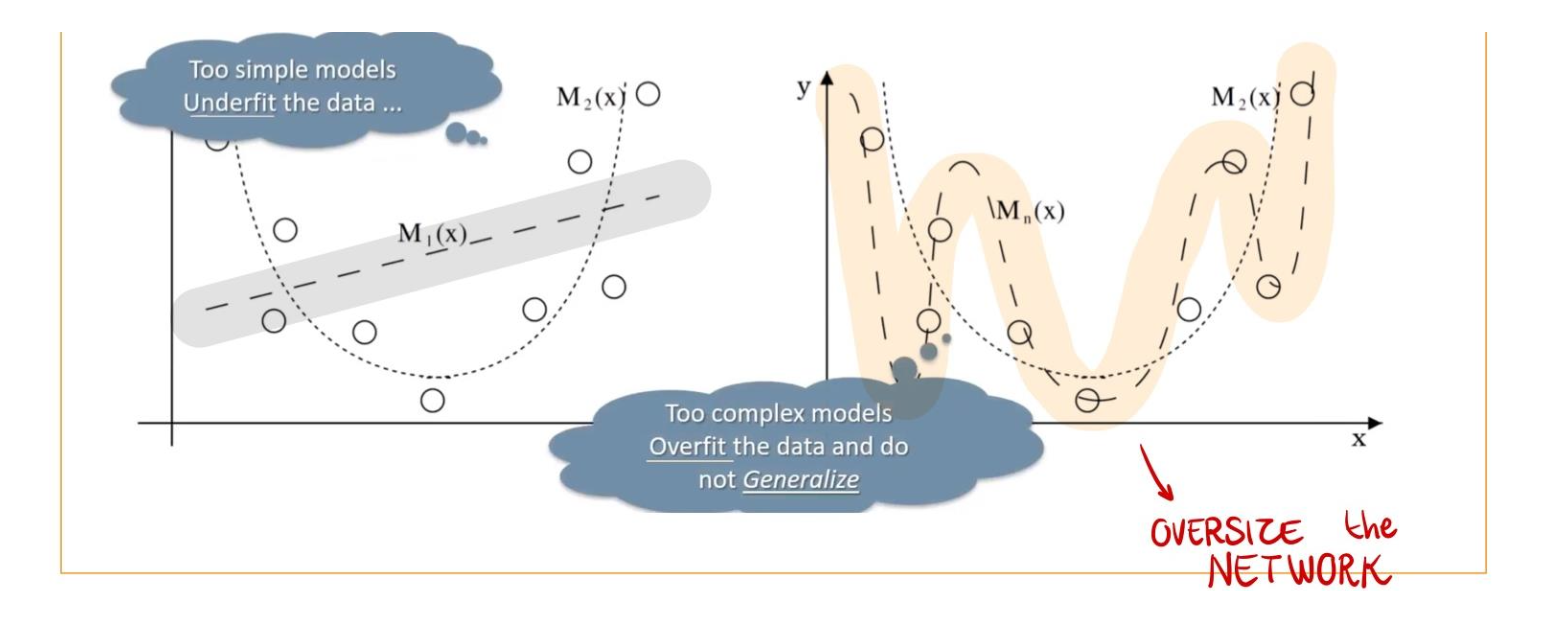
\includegraphics[width=\textwidth]{Images/overfitting_example.png}
        \caption{An example: polynomial curve fitting.}
    \end{figure}
    \end{column}
\end{columns}
\end{frame}

%------------------------------------------------------------
% SECTION: TRAIN AND TEST SET
%------------------------------------------------------------

\begin{frame}{The Data Splitting Rationale}
\begin{itemize}
    \item We want to measure a model's ability to generalize to new data.
    \item If we \textbf{evaluate} the model on the same data it was \textbf{trained} on:
    \begin{itemize}
       \item It may appear highly accurate due to overfitting.
       \item We get an overly optimistic measure of performance.
    \end{itemize}
    \item \textbf{Solution}: Split data into at least two sets:
    \begin{enumerate}
       \item \textbf{Training set}: for learning the model's parameters.
       \item \textbf{Test set}: for assessing generalization performance on \emph{unseen} data.
    \end{enumerate}
\end{itemize}
\end{frame}

%------------------------------------------------------------
% Slide: Visualizing Train-Test Split
%------------------------------------------------------------
\begin{frame}{Visualizing a Train-Test Split}
\begin{figure}
    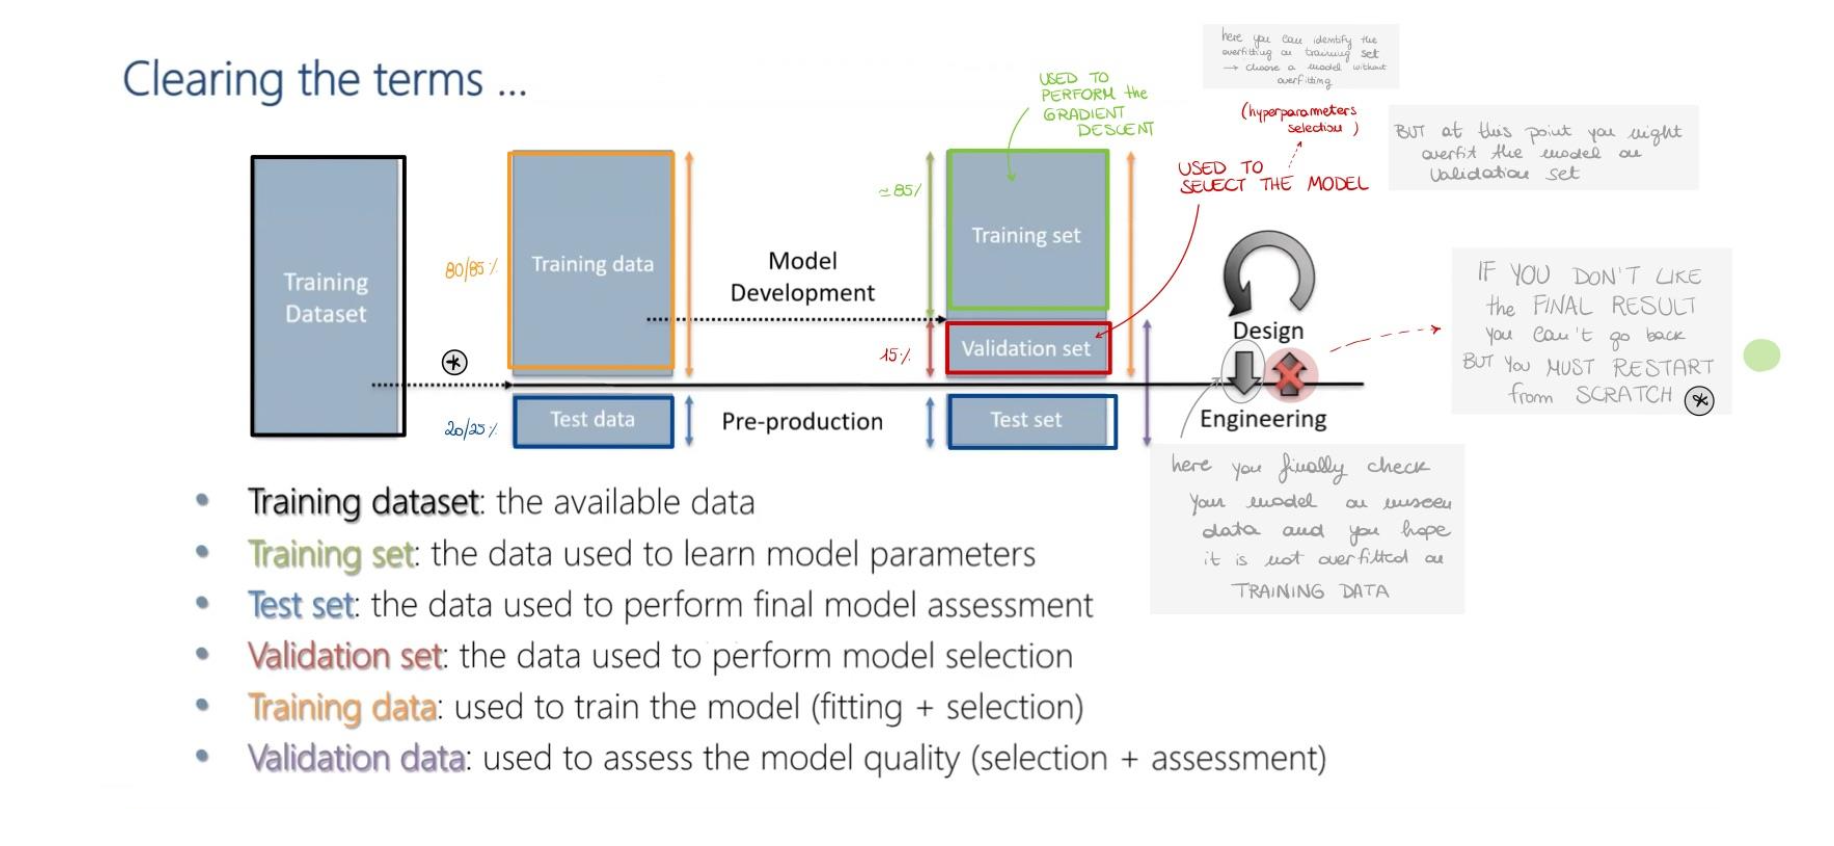
\includegraphics[width=\textwidth]{Images/train_test_split.png}
    \caption{A schematic view of dividing data into training and test sets.}
\end{figure}
\end{frame}

%------------------------------------------------------------
% Slide: How the Test Set Helps Prevent Overfitting
%------------------------------------------------------------
\begin{frame}{How the Test Set Helps Prevent Overfitting}
\begin{itemize}
    \item \textbf{Primary Goal}: Ensure that model evaluation is done on data the model has \textit{never} seen before.
    \item This gives a realistic estimate of how well the model might perform on real-world data.
    \item \textbf{Warning}: If you tweak the model repeatedly based on its performance on the test set, you risk overfitting to the test set itself. 
    \begin{itemize}
      \item A possible remedy is an additional \textbf{validation set} or using \textbf{cross-validation}.
    \end{itemize}
\end{itemize}
\end{frame}

% Slide 1: Introduction to Incomplete Data
\begin{frame}{1.1 Incomplete Data}
\textbf{Key Observation:} Datasets often contain \emph{missing values} for some attributes.

\begin{itemize}
  \item Missing values occur for many reasons: data collection errors, equipment failures, 
        user non-response, etc.
  \item Understanding different ways to handle missing data is crucial to avoid biased results.
\end{itemize}

\end{frame}

% Slide 2: Techniques to Partially Correct Incomplete Data
\begin{frame}{Techniques to Handle Missing Values}
There are several strategies to address missing data. Each has advantages and drawbacks:

\begin{enumerate}
  \item \textbf{Elimination (Case Deletion)}
  \begin{itemize}
    \item Discard all records for which one or more attributes are missing.
    \item \textit{Pros}: Simple to implement.
    \item \textit{Cons}: Can drastically reduce sample size and potentially introduce bias.
  \end{itemize}

  \vspace{0.2cm}

  \item \textbf{Inspection}
  \begin{itemize}
    \item Manually inspect and decide how to fill in each missing value.
    \item \textit{Pros}: Allows domain knowledge to guide the process.
    \item \textit{Cons}: Highly subjective and time-consuming.
  \end{itemize}
\end{enumerate}
\end{frame}

% Slide 3: Identification and Substitution
\begin{frame}{More Techniques for Missing Data}
\begin{enumerate}
  \setcounter{enumi}{2} % Continue numbering from previous slide

  \item \textbf{Identification}
    \begin{itemize}
      \item Use a conventional value (e.g., a special code) to denote missingness.
      \item \textit{Pros}: Keeps the record without discarding it entirely.
      \item \textit{Cons}: The special code might be interpreted as a real value if not handled carefully.
    \end{itemize}

  \vspace{0.3cm}

  \item \textbf{Substitution (Imputation)}
    \begin{itemize}
      \item Automatically replace missing data with a \textit{surrogate} value.
      \item Common approaches:
        \begin{itemize}
           \item Replace with the mean or median of the attribute (for numeric data).
           \item Replace with the mean of the attribute only within the same target class.
        \end{itemize}
      \item \textit{Pros}: Preserves the number of records.
      \item \textit{Cons}: Arbitrary, can distort distributions; more sophisticated methods (e.g., multiple imputation) might be needed.
    \end{itemize}

\end{enumerate}
\end{frame}

% Slide 4: Practical Considerations
\begin{frame}{Practical Considerations}
\begin{itemize}
  \item The \textbf{choice of technique} depends on:
  \begin{itemize}
    \item \textbf{Percentage of missing data} (low vs. high).
    \item \textbf{Type of attributes} (numeric vs. categorical).
    \item \textbf{Dataset size} and importance of each attribute.
    \item \textbf{Available domain knowledge}.
  \end{itemize}

  \item For large datasets with a high percentage of missing values:
  \begin{itemize}
    \item Manual inspection quickly becomes infeasible.
    \item Even mean-based imputation might be slow or simplistic.
    \item Advanced imputation methods (e.g., k-NN imputation, regression imputation, multiple imputation) may be considered.
  \end{itemize}
\end{itemize}
\end{frame}

